\section{Performance Suchalgorithmen}
\label{sec:testCenter.PerformanceSuchalgorithmen}

Die entwickelten Suchstrategien werden in diesem Kapitel verglichen. Zum Vergleich wird eine Testkarte der Gr�sse 100 x 110 Tiles verwendet, auf dieser werden die Pfadsuchalgorithmen angewendet. Die Suchstrategie \texttt{SIMPLE} wird nicht in den Vergleich einbezogen, diese ist wie beschrieben nur f�r kurze Pfade einsetzbar. Daf�r wird der HPA* mit zwei verschiedenen Clustergr�ssen (14 \& 20), sowie den unterschiedlichen Typen \texttt{Corner} und \texttt{Centered} angewendet. Der erste Test beinhaltet zwei Durchg�nge, bei welchen jeweils ein anderer Start- und Zielort definiert wurde.

\begin{table}[H]
	%weird hack to enable footnotes in the table
	\begin{minipage}{20cm}

		\begin{tabular}{ l | r  r  | r  r | r r }
		
		&  \multicolumn{2}{l|}{\textbf{1. Durchlauf}} & \multicolumn{2}{l|}{\textbf{2. Durchlauf}} &
		\multicolumn{2}{l}{\textbf{Durchschnitt}} \\
		
		\textbf{Suchalgorithmus} & \textbf{Dauer\footnote{Dauer in Millisekunden}} & \textbf{Pfadl�nge\footnote{Pfadl�nge in Anzahl Tiles}} & \textbf{Dauer} &
		\textbf{Pfadl�nge} & \textbf{Dauer} & \textbf{Pfadl�nge}  \\
		\hline
		
		A* & 124.6 & 95 & 101.2 & 95 & 112.9 &	95 \\
		HPA* (Centered,14)\footnote{Typ: Centered, Clustergr�sse: 14} & 167.6 & 99 & 25.2 & 107 & 96.4 & 103\\
		HPA* (Corner,14) & 2677.4 & 117 & 2394.6 & 117 & 2536 & 117 \\
		HPA* (Centered,20)  & 6.4 & 106 & 60 & 137 & 33.2 & 121.5 \\
		HPA* (Corner,20) & 22 & 113 & 231 & 133 & 126.5 & 123 \\
		\end{tabular}\par
		\vspace{-0.75\skip\footins}
   \renewcommand{\footnoterule}{}
  \end{minipage}
	\caption{Testresultate: Vergleich der Suchalgorithmen}
	\label{tab:testSearchAlgorithms}
\end{table}



In der Tabelle \ref{tab:testSearchAlgorithms} sind die Testresultate aufgelistet. Zu sehen ist, dass nur A* den optimalen Pfad von 95 \gls{Tile}s findet, und zwar in ca. 120 Millisekunden. HPA* mit Typ \texttt{Corner} und mit der kleinerer Clustergr�sse von 14 \gls{Tile}s ist langsamer als A*. Dies ist darauf zur�ckzuf�hren, dass mit dieser Einstellung das Clusternetz von HPA* zu feinmaschig ist. Um den Pfad zu finden m�ssen viele Kanten und Knoten der geclusterten Karte durchforscht werden. Das dauert l�nger als bei A*, wo die Nachfolgerknoten einfach aus einem zweidimensionalen Array gelesen werden.

Der Typ \texttt{Centered} ist deutlich schneller als der Typ \texttt{Corner}, da er in etwa nur halb so viele Pfadknoten pr�fen muss (siehe Kapitel \ref{subsec:module.Suchalgorithmen.Pfadsuche.HPAstar}). Sobald die Clustergr�sse auf 20 \gls{Tile}s gestellt wird, ist HPA* deutlich schneller als A*. Allgemein muss aber gesagt werden, dass es sehr darauf an kommt, ob die Gel�ndestruktur dem Clustering entgegenkommt, so dass die Verbindungspunkte g�nstig gelegen sind und ein Pfad gefunden werden kann, der nicht zu viele Umwege macht. Abbildung \ref{fig:comapreSearchStrategies} zeigt, wie die verschiedenen Suchalgorithmen den Pfad zwischen den zwei schwarzen Punkten gefunden haben.

\begin{figure}[H]
\centering
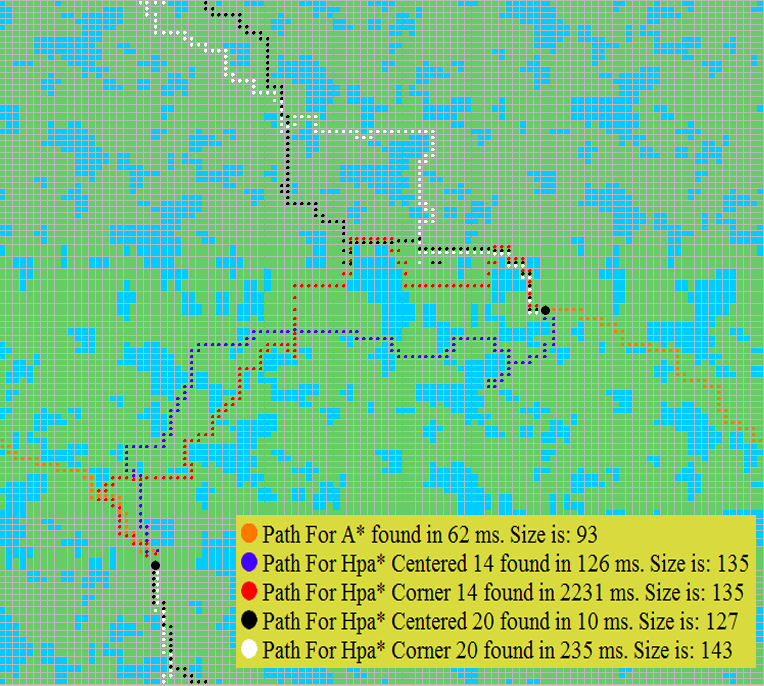
\includegraphics[height=100mm]{91_bilder/searchcompare}
\caption[Vergleich der Suchalgorithmen]{Vergleich der gefundenen Pfade: Viele Wege f�hren nach Rom.}
\label{fig:comapreSearchStrategies}
\end{figure}

Beim ersten Test wurde der Pfad nicht gesmoothed, und auch die Zeit, welche es brauchte um die Karte in Cluster aufzuteilen, ist nicht ber�cksichtigt. Nachfolgender Test ber�cksichtigt nun diese zwei Aspekte.

\begin{table}[H]
	%weird hack to enable footnotes in the table
	\begin{minipage}{11cm}

		\begin{tabular}{ l | r r r r r }
		
		\textbf{Suchalgorithmus} & \textbf{Clustering} & \textbf{Pfadsuche} & \textbf{PathSmoothing} & 
		\textbf{Pfadl�nge 1}\footnote{ohne Smoothing} & \textbf{Pfadl�nge 2}\footnote{mit Smoothing}  \\
		\hline		
		A* & - & 95 ms & - & 95 & -  \\
		HPA* (Centered,20)  & 484 ms & 4 ms & 16 ms & 127 & 119 \\
		\end{tabular}\par
		\vspace{-0.75\skip\footins}
   \renewcommand{\footnoterule}{}
  \end{minipage}
	\caption[Testresultate: Vergleich der Suchalgorithmen mit PathSmoothing]{Testresultate: Dauer, mit Ber�cksichtigung von Clustering und PathSmoothing}
	\label{tab:totalDuration}
\end{table}

Um die Cluster f�r die ganze Karte zu berechnen, braucht es einmalig ungef�hr 480 Millisekunden. Weil in einem konkreten Spiel die Karte nur nach und nach erkundet wird, verteilt sich der Aufwand f�r das Clustering auf mehrere Z�ge und ist deswegen f�r uns nicht kritisch. Wenn wir einen gegl�tteten HPA* wollen, brauchen wir ca. 20 ms pro Suche; f�r den optimalen Pfad mit A* 95 ms. Mit der Verwendung von HPA* sparen wir also im Schnitt rund 70 ms pro Pfadsuche. Wenn man ber�cksichtigt, dass pro Zug f�r mehrere Ameisen ein Pfad gesucht wird, lohnt sich der Einsatz von HPA* allemal.